\chapter{Chromatin is globally compacted upon local damage, with nodes of repair in decondensed regions}

\paragraph*{} The advantage of FAI is in the fact that it could be useful for observing chromatin dynamics in live and fixed cells. Since I have introduced a 405nm laser in our widefield setup with the dual lamp housing (Fig. {\ref{fig:setup}}), I could microirradiate specific regions in hoechst-sensitized HeLa H2B-EGFP cells, and cause a localized damage, and monitor the change in the global state of chromatin compaction. Using DNA damage markers, I followed damage repair dynamics along with chromatin compaction states. 

\section{Microirradiation induced damage}

\paragraph*{} To test that the 405nm laser that is introduced using the DLH is performing as intended, I focused the laser to a diffraction limited spot in the center of the image plane, and irradiated hoechst-sensitized cells. I observed that it causes damage by fixing the damaged cell within 5 minutes and staining the microirradiated cell for $\gamma$H2AX, which was observed at the site of damage (Fig. {\ref{fig:micro_gh2ax}}), indicating activated damage response.

\begin{figure}[!htp]
    {\hfill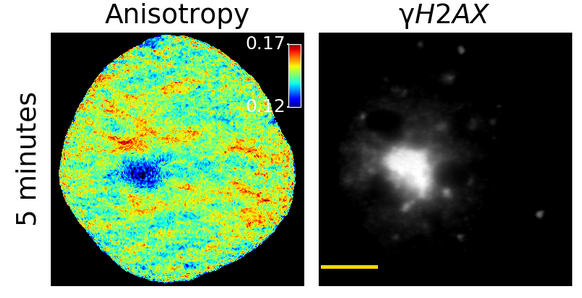
\includegraphics[clip,width=0.8\linewidth]{figures/micro_gh2ax.png}\hspace*{\fill}}
    \caption{Microirradiation activates DNA damage responses. $\gamma$H2AX, a known marker for damage response, is found at the site of microirradiation.}
    {\label{fig:micro_gh2ax}}
\end{figure}


\begin{figure}[!htp]
    {\hfill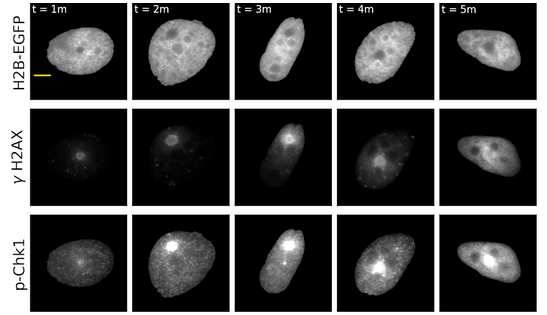
\includegraphics[clip,width=1\linewidth]{figures/pchk1.png}\hspace*{\fill}}
    \caption{Pan-nuclear induction of $\gamma$H2A.X in response to laser microirradiation. Hoechst-sensitized cells were microirradiated at intervals of 1 minute, with a different cell being irradiated every minute. Cells are fixed and stained for markers of damage response, $\gamma$H2A.X and phospho-Chk1 (a target of the ATR kinase). These are representative cells, but generally too induction of $\gamma$H2A.X is seen at the site of damage at the early timepoints, but it spreads out and there is pan-nuclear $\gamma$H2A.X induction 5-10 minutes onwards. Phospho-Chk1 is still enriched at the site of damage even at these later time-points. Scalebar is 5$\mu$m.}
    {\label{fig:chk1}}
\end{figure}


\paragraph*{} I intended to use fluorescence anisotropy imaging to study the changes to chromatin structure that has undergone microirradiation induced DSBs as employed by previous studies \cite{kruhlak2006changes, BURGESS20141703,strickfaden2016poly}. With the modified FAI microscope with a 405-nm laser into the light path and Hoechst-sensitized cells were used to cause local double-strand breaks of the DNA. Minutes after irradiation, strong staining for $\gamma$H2AX and the phosphorylated form of Chk1 (p-Chk1, a target of the master DDR kinase ATR) was observed at the site of damage (Fig. {\ref{fig:chk1}}), which indicated that the damage response was in action. 


\paragraph*{} I noticed that within 1 min after microirradiation, there is phosphorylation of Ser139 of the histone variant H2AX at the site of microirradiation, indicating DNA damage. Although $\gamma$H2AX is a DNA damage marker, which is generally found as foci in regions of damaged chromatin, there is also a pan-nuclear spreading of $\gamma$H2AX in undamaged chromatin as early as 5 min after damage. 

\paragraph*{} In another study, interference with chromatin compaction at the damage site reduces the efficiency of damage repair. This suggested that condensation of chromatin is a necessary step in the activation of DDR \cite{BURGESS20141703}. However, ATM activation in mouse fibroblasts showed chromatin opening independent of DNA damage \cite{ji2017baf60b}. During damage, ATM is thought to be activated not by direct binding to DNA strand breaks, but by changes in chromatin structure. Thus, forced compaction of chromatin promotes activation of ATR and ATM even where there are no strand breaks \cite{BURGESS20141703}, and conversely, activation of these kinases can change chromatin compaction \cite{becker2014atm}. Thus, pan-nuclear induction of DDR (for which $\gamma$H2AX is a proxy) can drive compaction of undamaged chromatin, and the processes could feed back onto each other.

\paragraph*{} Such pan-nuclear induction of $\gamma$H2AX has been reported before when clustered DNA damage was induced by ionizing radiation, which is regulated by ATM and DNA-PK \cite{meyer2013clustered}. Other studies have discussed a ring of $\gamma$H2AX in the context of apoptosis \cite{solier2014nuclear}. It is possible that some of the cells I have irradiated will undergo apoptosis, and apoptotic response over and above the DNA damage response complicates the observed chromatin phenotypes.

\begin{figure}[H]
    {\hfill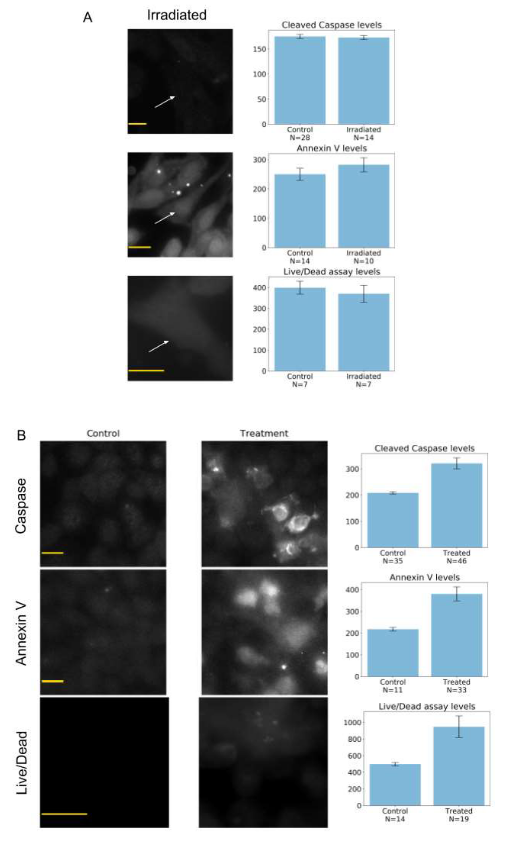
\includegraphics[clip,width=0.8\linewidth]{figures/apoptosis.png}\hspace*{\fill}}
    \caption{Apoptosis markers are absent in irradiated cells compared to control unirradiated cells. Apoptosis was probed with different markers (A) Cleaved Caspase 3, Annexin V or Live/Dead assay with the intensity of the relevant cell death marker quantified. Irradiated cells (marked with white arrow) show similar to control level of marker staining, indicating the
    absence of apoptotic response, as quantified on the right for several cells. (B) As a positive control to show that the reagents are working, we used staurosporine-treated (1 $\mu$M, 4 hrs) cells, which do show an induction of the cell death marker in all three cases. Error bars indicate standard error of mean. Scale bar is 15$\mu$m}
    {\label{fig:apoptosis}}
\end{figure}


\paragraph*{} However, apoptosis is accompanied by visible changes in the cell and nuclear morphology. However, our irradiated cells, under similar irradiation conditions, do not exhibit apoptotic morphology or fragmented chromatin, and many survive 48 h after irradiation. Furthermore, during the time course over which the cells were imaged in our study, there was no significant induction of apoptotic or general cell death markers (Fig. {\ref{fig:apoptosis}}). This indicates that the effects I observe may have to do with the early processes of DDR rather than the long-term processes of cell death because of excessive DNA damage.


\section{Chromatin dynamics upon damage}
\begin{figure}[!htp]
    {\hfill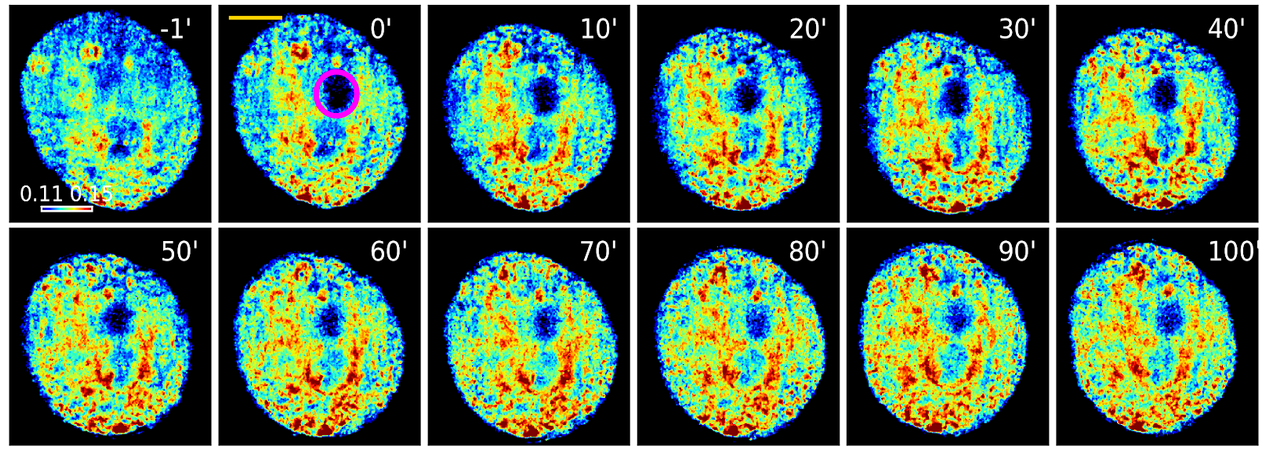
\includegraphics[clip,width=1\linewidth]{figures/live_an.png}\hspace*{\fill}}
    \caption{Dense nodes of chromatin are formed in microirradiated cells. H2B-EGFP anisotropy time series for a representative irradiated cell before and after irradiation, imaged every 5 min for over 2 h. The color map is scaled from 0.11 to 0.15. Scale bar corresponds to 5$\mu$m. Magenta circles indicate the sites of microirradiation.}
    {\label{fig:live_an}}
\end{figure}

\paragraph*{} Using this microirradiation protocol, I collected anisotropy data for the damaged cells over a period of 2 h, imaged once every 5 min (Fig. {\ref{fig:live_an}}). Anisotropy at the site of the damage could not be ascertained due to localized photobleaching of H2B-EGFP upon irradiation, but the response of the rest of the chromatin, which did not see direct irradiation, could be followed. 


\begin{figure}[H]
    {\hfill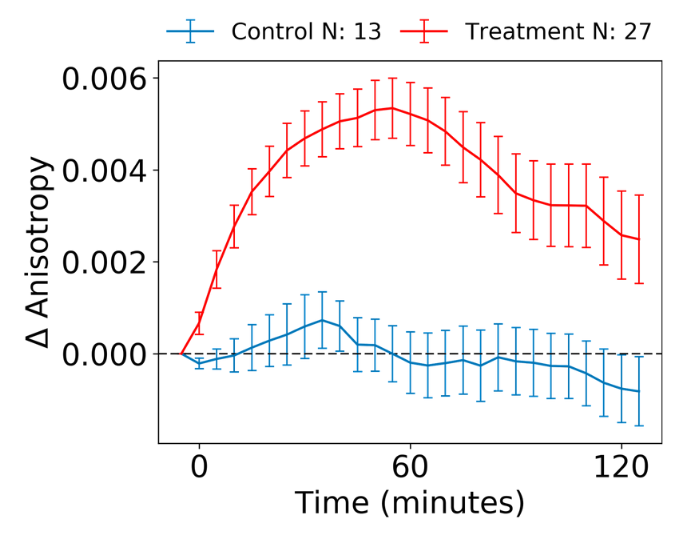
\includegraphics[clip, width=0.5\linewidth]{figures/timetrace.png}\hspace*{\fill}}
    \caption{$\Delta$Anisotropy is calculated by subtracting the mean anisotropy of any time point, with the mean anisotropy of the first time point for that cell. A positive $\Delta$Anisotropy corresponds to compaction, whereas a negative $\Delta$Anisotropy corresponds to decompaction.}
    {\label{fig:timetrace}}
\end{figure}

\paragraph*{}In comparison to the control undamaged cells (N = 13), the overall $\Delta$anisotropy value ($\Delta$anisotropy = rt – r0, where rt is the mean anisotropy at any given time point, and r0 is the mean anisotropy for the 0th time point) of the irradiated cells increased with time (Fig. {\ref{fig:timetrace}}), though the response was heterogeneous among cells ((Fig. {\ref{fig:hetero}})). And though the mean rise is small, one should keep in mind that anisotropy values are themselves fractional; also, mean anisotropy averages over regions where compaction increases and surrounding regions where it decreases correspondingly, keeping the changes in mean anisotropy small. This heterogeneity is captured in the anisotropy maps, and indeed a fraction of cells show formation of nodes of high local compaction even in regions that have not directly been damaged (Fig. {\ref{fig:live_an}}). 

\begin{figure}[htp]
    {\hfill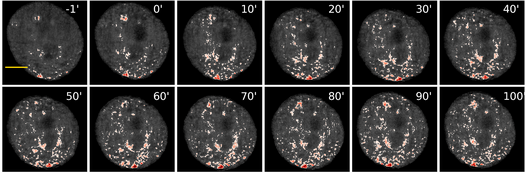
\includegraphics[clip, width=1\linewidth]{figures/thresholded.png}\hspace*{\fill}}
    \caption{A gray anisotropy map is plotted with color for anisotropy values greater than a threshold (mean + 2*standard deviation) calculated with respect to the -1' timepoint. The fraction of pixels above this constant threshold calculated for the -1' timepoint visibly grows with time indicating local compaction. Scale bar corresponds to 5$\mu$m.}
    {\label{fig:thresholded}}
\end{figure}

\paragraph*{} To quantify this better and visualize the nodes, I thresholded the anisotropy map with a threshold value of “mean + 2 $\sigma$,” where mean is the mean anisotropy value of the nucleus before damage and $\sigma$ is the standard deviation of the mean. Values below the threshold are turned to gray, so that it becomes easier to visualize the high–anisotropy value pixels formed upon irradiation (Fig. {\ref{fig:thresholded}}). 

\paragraph*{} The formation of high-anisotropy nodes is reflected in the overall increase in high-anisotropy pixels for irradiated cells as compared with control cells. However, it should be noted that the control cells also show a fair degree of heterogeneity among themselves, and this could be because of toxic effects of the imaging excitation light, natural cell cycle–driven processes that causes chromatin compaction changes, or systematic changes to anisotropy with photobleaching. 


\begin{figure}[H]
    {\hfill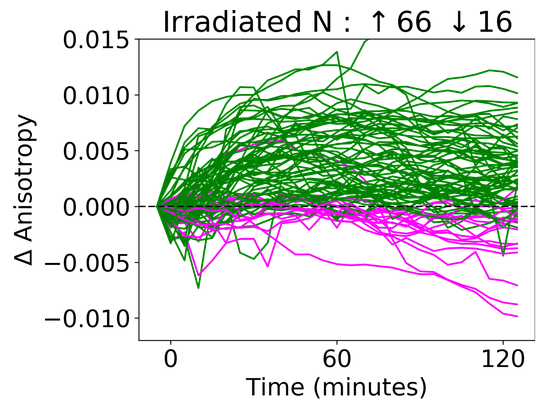
\includegraphics[clip, width=0.8\linewidth]{figures/closely.png}\hspace*{\fill}}
    \caption{Pooled single cell traces for irradiated cells done on three different days. 66 show a positive (green) trend and 16 a negative (magenta) trend.}
    {\label{fig:closely}}
\end{figure}


\paragraph*{} Nonetheless, the propensity for increased compaction in irradiated cells is clear and significantly different from the dynamics of control cells. When the individual $\Delta$anisotropy time trace for each irradiated cell is examined closely (Fig. {\ref{fig:closely}}), 21 out of 27 cells show positive increase in delta anisotropy and only 6 out of 27 cells show an overall negative trend over the 2 h after damage, whereas in control cells, 7 out of 13 cells show a positive trend and 6 out of 13 cells show a negative trend. This indicates that there is inherent variability in the cellular response to damage, but overall there is condensation of chromatin in response to damage.



\begin{figure}[!htp]
    {\hfill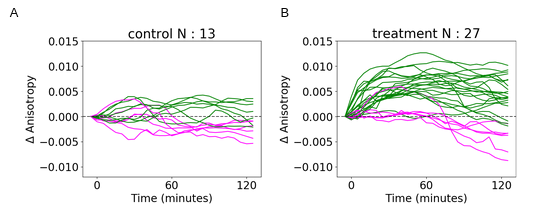
\includegraphics[clip, width=1\linewidth]{figures/hetero.png}\hspace*{\fill}}
    \caption{Compaction of undamaged chromatin in response to local damage.Individual $\Delta$anisotropy time traces of A. control (13 cells) and B. irradiated cells (27 cells). Cells with an overall positive trend are color-coded green, while those with a negative trend color-coded magenta. }
    {\label{fig:hetero}}
\end{figure}

\begin{figure}[!htp]
    {\hfill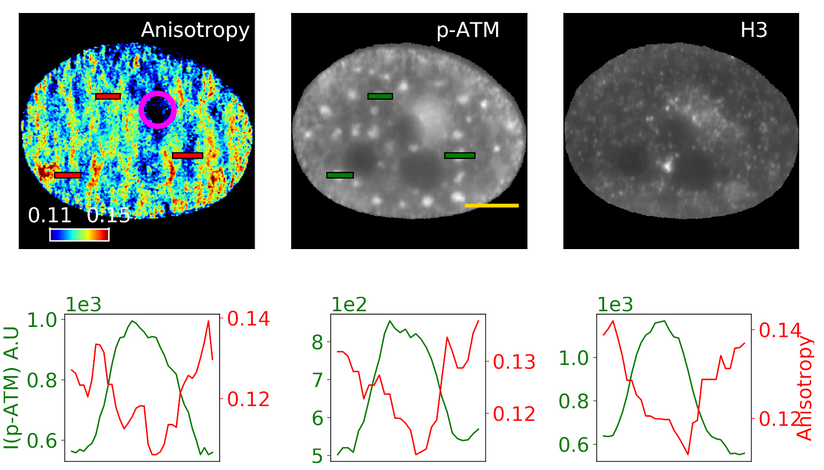
\includegraphics[clip, width=1\linewidth]{figures/patm.png}\hspace*{\fill}}
    \caption{Microirradiated cells are fixed after live imaging, and stained for damage markers. Phosphorylated-ATM is seen at sites of low anisotropy regions, and Histone H3 is accumulated at the site of damage. The purple circle is the site of microirradiation.}
    {\label{fig:patm}}
\end{figure}

\section{Live-cell detection of damage markers with chromatin dynamics}

\paragraph*{}  Next I wanted to combine the time course of anisotropy imaging with live-cell detection of other markers of the damage response. For this, I chose chromobody-mediated detection of early and late markers of DDR—PARP1 and PCNA. PARP1 is known to be transiently enhanced at sites of damage in response to irradiation-induced DSBs \cite{chou2010chromatin,qi2019multiple}, while PCNA, being the DNA clamp, would be required for the processivity of the DNA polymerase in the final steps of repair \cite{moldovan2007pcna}. 

\paragraph*{} I independently transfected PARP1 and PCNA chromobodies tagged with TagRFP in HeLa cells stably expressing H2B-EGFP. Chromobodies (ChromoTek) are small intracellular antibodies tagged with fluorescent protein. Their major advantage is that they detect the endogenous proteins they are designed against without artifacts of overexpression of those proteins in transient transfections \cite{BURGESS20141703,panza2015live}.

\begin{figure}[H]
    {\hfill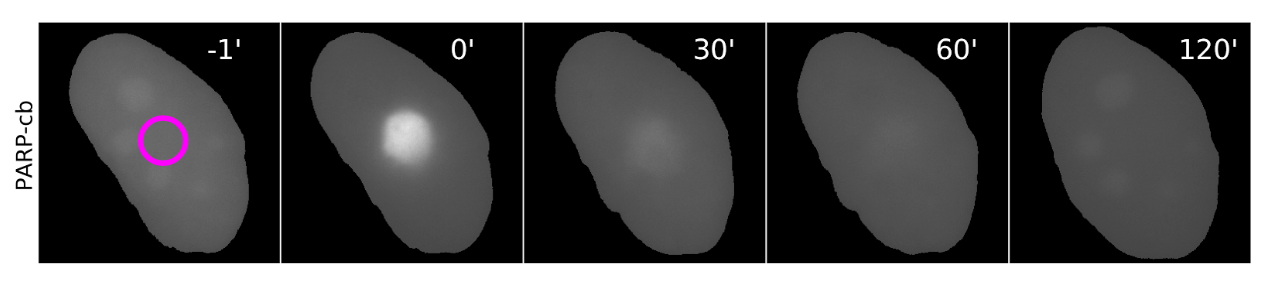
\includegraphics[clip, width=1\linewidth]{figures/parp.png}\hspace*{\fill}}
    \caption{Live cell dynamics of PARP-chrombody in irradiated cells, transiently transfected in HeLa H2B-EGFP cells. PARP1 showed immediate transient encrichment at the site of damage, and became homogenous quickly.}
    {\label{fig:parp}}
\end{figure}

\paragraph*{} As expected, PARP1 was recruited to the site of damage almost immediately upon irradiation (Fig. \ref{fig:parp}). However, the PARP1 signal diffused away from the site by 15 min after damage, as expected \cite{haince2008parp1,mortusewicz2007feedback}. 


\begin{figure}[H]
    {\hfill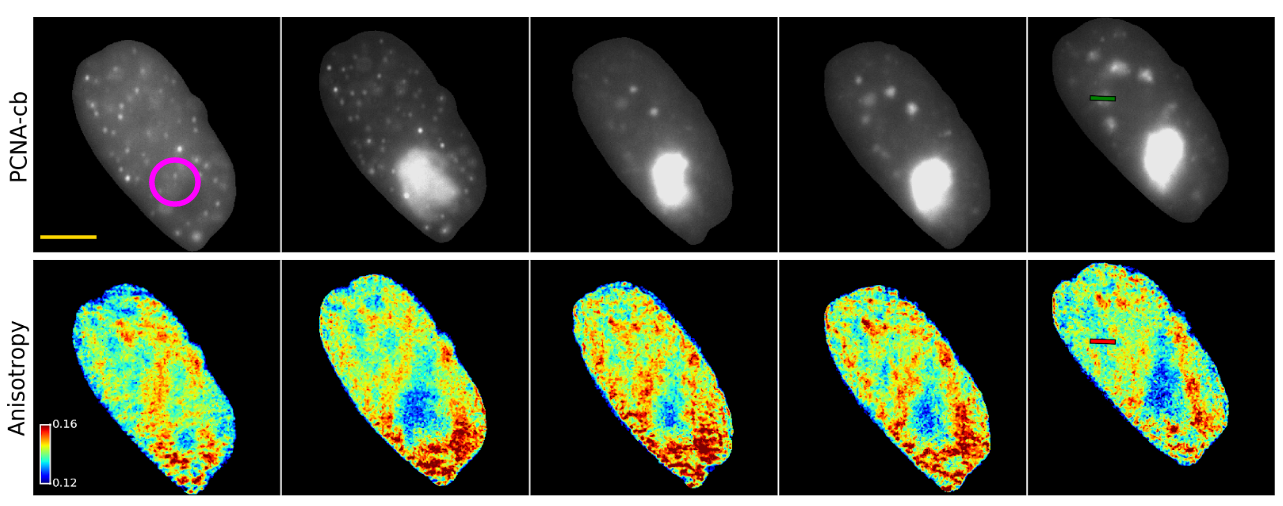
\includegraphics[clip, width=1\linewidth]{figures/pcna.png}\hspace*{\fill}}
    \caption{HeLa H2B-EGFP cells expressing PCNA chromobody along with its corresponding anisotropy maps, imaged at an  interval of 5 minutes post-irradiation. Scale bar corresponds to 5$\mu$m. Timestamps are same as (Fig. \ref{fig:parp})}
    {\label{fig:pcna}}
\end{figure}

\paragraph*{} It was surprising to note, PCNA, which should be involved in the repair only at later stages, was also recruited immediately to the site of damage (Fig \ref{fig:pcna}). This was the case in G1 and G2 cells where the PCNA chromobody was homogenous in the nucleus, and even in S phase cells where the PCNA chromobody was punctated, as PCNA follows the replication fork. The PCNA chromobody is primarily used for cell-cycle stage detection \cite{BURGESS20141703}. This implies that in response to clustered DSBs, even PCNA from replication forks is recruited to the site of damage. 


\begin{figure}[H]
    {\hfill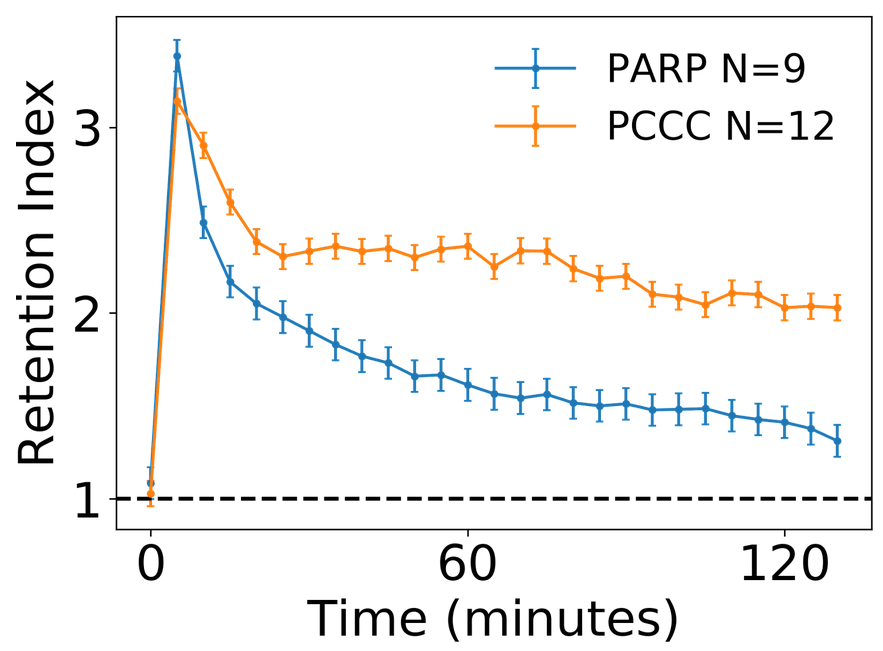
\includegraphics[clip, width=0.5\linewidth]{figures/retention.png}\hspace*{\fill}}
    \caption{PCNA persists at the site of damage longer than PARP. Retention index of any time point is defined as the ratio of intensity for a chromobody at the site of damage and outside the site of damage.}
    {\label{fig:retention}}
\end{figure}

\paragraph*{} PCNA persisted at the site of damage for the duration of the time course, longer than PARP1 (Fig. \ref{fig:retention}). This local enrichment was quantified by plotting the mean intensity of the chromobody at the site of damage normalized to the mean intensity outside. I found this to be a more robust metric for the enrichment, compared with just the normalized intensity at the site of damage, which decays due to photobleaching during the time course, in addition to actual dynamics. This metric is more robust because photobleaching operates both within and outside the site of damage. 

\begin{figure}[H]
    {\hfill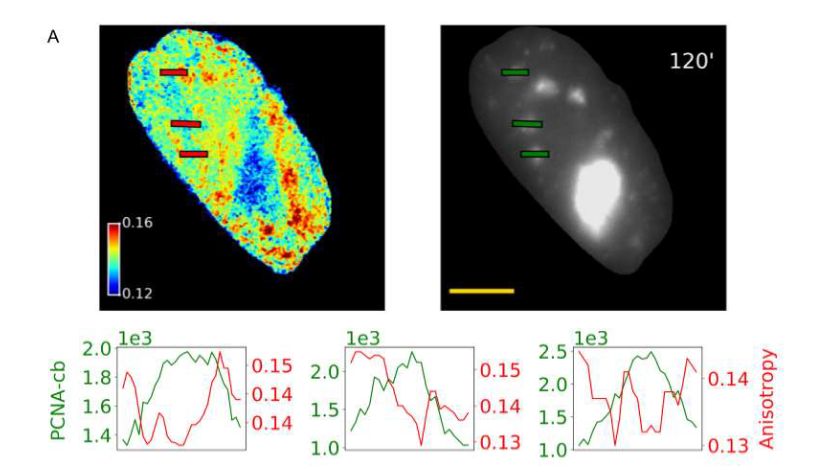
\includegraphics[clip, width=1\linewidth]{figures/node.png}\hspace*{\fill}}
    \caption{PCNA transient nodes form in low anisotropy regions. Anisotropy map of an irradiated cell which is transfected with PCNA chromobody shows local transient enrichment of PCNA at low anisotropy regions at the 120 minute timepoint, as shown by line profiles. Lines are shown in red on the anisotropy map and green in PCNA image. Scale bar corresponds to 5$\mu$m.}
    {\label{fig:node}}
\end{figure}

\paragraph*{} However, while PCNA persists longer, within 20 min, there are nodes of PCNA formed, away from the site of damage, which correspond to regions of lower anisotropy (Fig. \ref{fig:node}). I asked whether these sites of PCNA enrichment and low anisotropy represent simply sites of repair factor storage or of active repair. I reasoned that if they are indeed sites of repair, even in the G1 or G2 phase, I may be able to see incorporation of a deoxynucleotide analog such as ethynyl deoxyuridine (EdU). 


\begin{figure}[htp]
    {\hfill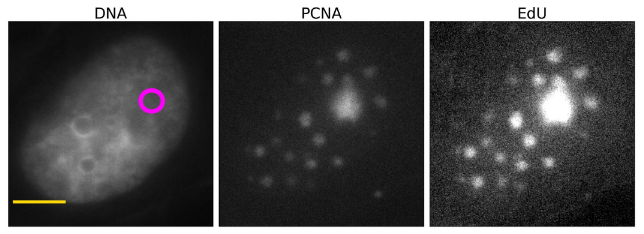
\includegraphics[clip, width=1\linewidth]{figures/edu.png}\hspace*{\fill}}
    \caption{Sites of PCNA accumulation show EdU incorporation even outside the site of damage. Images of DNA stained with Hoechst, PCNA chromobody labeled with TagRFP, and EdU detected with Cy5 Azide are shown. The magenta circles indicate sites of microirradiation-induced damage. Scale bar corresponds to 5$\mu$m.}
    {\label{fig:edu}}
\end{figure}

\paragraph*{} HeLa cells transfected with the PCNA chromobody were subjected to laser-induced DSBs. G1 or G2 cells that have a homogenous distribution of the PCNA chromobody in the nucleus were chosen. I observed that at these sites of transient PCNA nodes, EdU is incorporated, which is an indication of new DNA being synthesized at these sites (Fig. \ref{fig:edu}). 

\begin{figure}[htp]
    {\hfill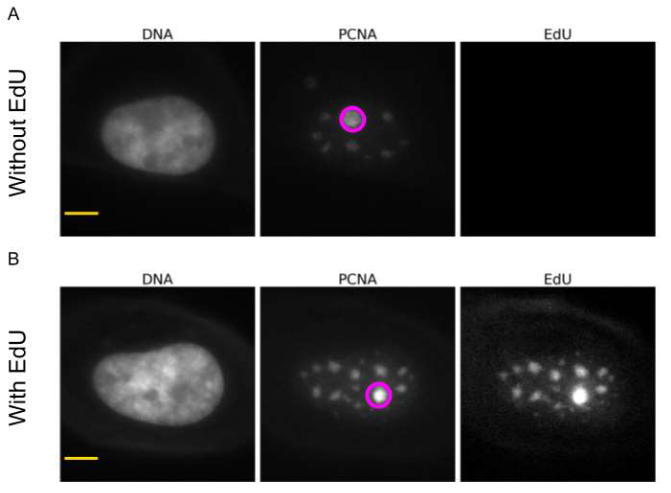
\includegraphics[clip, width=1\linewidth]{figures/bleed.png}\hspace*{\fill}}
    \caption{PCNA does not bleedthrough into EdU channel. HeLa cells transfected with the PCNA chromobody A. without EdU in the FluoroBrite imaging medium, or B. with EdU in the FluoroBrite imaging medium. Cells were processed and imaged simultaneously under identical conditions. While PCNA transient PCNA nodes were seen in both cases (expression levels varied from cell to cell), no EdU signal was seen in the A. This shows that the EdU signal colocalizing at the sites of PCNA enrichment is not bleedthrough from PCNA channel. Scale bars represent 5$\mu$m and the site of damage is marked with a magenta circle. Representative examples of cells with DNA stained with Hoechst, PCNA chromobody labeled with TagRFP and EdU detected with Cy5 Azide are shown.}
    {\label{fig:bleed}}
\end{figure}

\paragraph*{} I ruled out bleedthrough of PCNA signal in the EdU channel by imaging plates for cells with and without EdU treatment (Fig. \ref{fig:bleed}). Thus, though the DSBs are induced locally, these nodes of PCNA incorporating EdU further away may indicate a looping out of individual DSBs from the site of primary damage.

\paragraph*{} This study establishes the possibility of using FAI to measure chromatin compaction changes in the context of DNA damage in living cells, followed by immunofluorescence for DDR and chromatin markers. While the response to DSBs is investigated here, following previous studies \cite{kruhlak2006changes,BURGESS20141703}, in principle, the method is amenable to other forms of DNA damage as well, which can be further investigated in the future.

\paragraph*{} In the context of DDR, these fluorescence anisotropy imaging studies suggest that the undamaged chromatin is globally compacted in response to localized DSB damage. In regions away from the site of damage, I observe chromatin nodes forming, as well as transient accumulation of phospho-ATM and PCNA in specific sites that correspond to more loosely packed regions of chromatin. These low-anisotropy regions with accumulated repair proteins could be regions of repair or of factors poised for repair. 

\begin{figure}[htp]
    {\hfill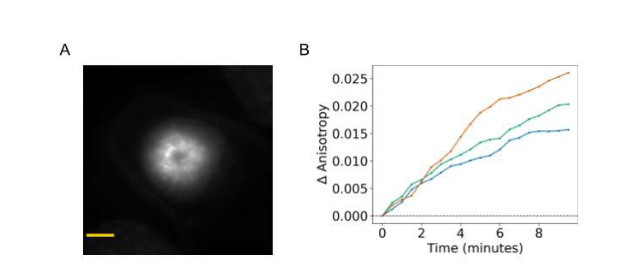
\includegraphics[clip, width=1\linewidth]{figures/pagfp.png}\hspace*{\fill}}
    \caption{H2B-PA-GFP activated, and irradiated with 405nm laser, shows increased anisotropy in a shorter period of time. A. Representative image of an activated H2B-PA-GFP exhibiting fluorescence in the GFP channel upon irradiation with 405 nm laser at the site of damage. B. Individual $\Delta$anisotropy time traces of three damaged H2B-PA-GFP expressing cells showing local increase in anisotropy and hence chromatin compaction. In this experiment there was a difference of less than 5 mins among the microirradiation of different cells and the start of anisotropy imaging (timepoint 0). All three cells show a trend of increasing anisotropy. The scalebar is 5 $\mu$m.}
    {\label{fig:pagfp}}
\end{figure}


\paragraph*{} A limitation of this technique is that I follow the response of undamaged chromatin because of local clustered DSBs, but anisotropy information is lost at the site of damage because of photobleaching. This could potentially be circumvented by using a histone H2B tagged with photoactivable GFP (H2B-PA-GFP). Condensation of the damaged chromatin could indeed be observed in such an experiment (Fig. \ref{fig:pagfp}). Using a procured plasmid for expressing H2B-PA-GFP in cells, as done in previous studies (Addgene plasmid No. 33000) \cite{kruhlak2006changes}. Since the same 405 nm laser line is used both for photoactivation of PA-GFP, and also for causing damage in Hoechst-sensitized cells, I reasoned that this would let us follow the compaction changes at the site of damage. I transiently transfected HeLa cells with this construct, and indeed could photoactivate H2B-PA-GFP and damage chromatin at the same site. Hoechst-sensitized HeLa cells expressing H2B-PA-GFP were microirradiated with the 405 nm laser to damage a site in the nucleus, while simultaneously activating the GFP at the site. I observed that the photoactivated region shows increased anisotropy over minutes, signifying condensation at the site of DNA damage following microirradiation


\paragraph*{} Another major limitation that I realized while performing the experiments in this chapter was the challenges posed by the microscope software as I set to improve the sample size for any given experiments. There were problems related to manual screening for suitable cells to damage and monitore further, which took long hours, as the cells had to express enough H2B-EGFP to have sufficient signal in the detector, for a given exposure, while also not express the protein in large amount so as to saturate the detector. There was also the danger of bleaching the sample during manual observation, which could lead to lower signal, and phototoxic artificats. It was necessary to have a system that could automatically identify and screen cells. Besides, I wanted to automate the screening so that while reducing time and effort in setting up the experiment, it could also null the effects of human bias, that are usually introduced in manual selection, in future experiments which require picking cells for observation. However, to incorporate such features into the experimental process, it required me to develop a microscope control software from scratch, which is detailed in the next chapter. 

